\subsection{ข้อแตกต่างระหว่างโครงสร้างของมนุษย์กับโครงสร้างของหุ่นยนต์}

\subsubsection{ความแตกต่างขององศาเสรี}
เนื่องจากลักษณะข้อต่อของมนุษย์มีความซับซ้อนมากกว่าโครงสร้างของหุ่นยนต์
ทำให้ข้อต่อแต่ละจุดของมนุษย์นั้นสามารถหมุนได้หลายทิศทาง รวมถึงขอบเขตของการหมุนของข้อต่อในแต่จุดก็มีความแตกต่างกัน
ในการนำรูปแบบการเดินของมนุษย์ไปใช้กับหุ่นยนต์จึงต้องปรับค่ามุมที่ข้อต่อให้มีความเหมาะสมกับโครงสร้าง
และข้อจำกัดเกี่ยวกับการหมุนของข้อต่อจุดต่างๆของหุ่นยนต์ที่จะใช้ทดสอบด้วย

\subsubsection{ความแตกต่างของอัตราส่วน}
นอกจากความแตกต่างขององศาเสรี (DoF) ระหว่างมนุษย์กับหุ่นยนต์แล้ว
ความแตกต่างของอัตราส่วนระหว่างโครงสร้างแต่ละส่วนของมนุษย์กับหุ่นยนต์เป็นอีกสาเหตุหนึ่ง
ที่ต้องทำการปรับแต่งใหม่มีความเหมาะสม เนื่องจากความยาวของโครงสร้างแต่ละส่วน
รวมทั้งระยะห่างระหว่างจุดหมุนแต่ละจุดของมนุษย์กับหุ่นยนต์ที่มีความแตกต่างกัน
ดังนั้นจึงต้องกำหนดระบบพิกัดเพื่อใช้อ้างอิงจุดหมุนและความยาวของโครงสร้าง
\begin{figure}[H]
    \centering
    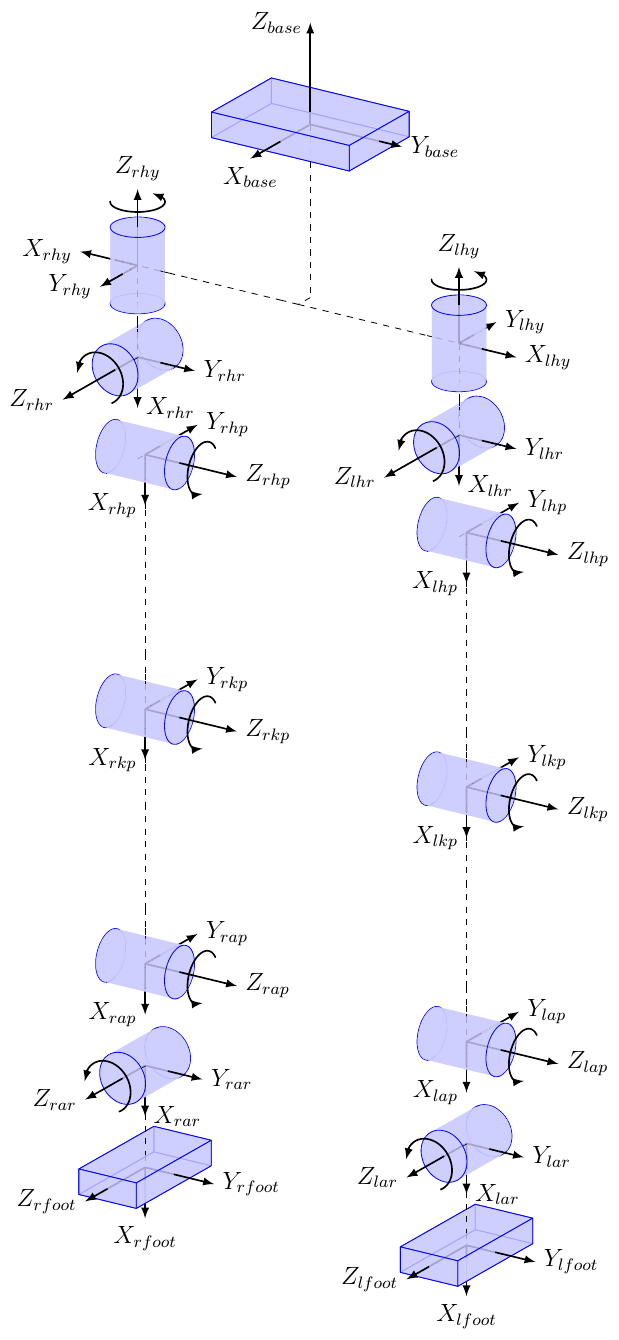
\includegraphics[width=0.25\textwidth]{chapter2/images/uthai_kinematics.png}
    \caption{ตัวอย่างตำแหน่งและการหมุนของข้อต่อของหุ่นยนต์เพื่อการอ้างอิง}
    \label{fig:robot_frame}
\end{figure}


\subsubsection{กำลังและประสิทธิภาพของมอเตอร์}
ความสามารถในการรับน้ำหนักของข้อต่อแต่ละจุดมีความแตกต่างกัน การเคลื่อนไหวของมนุษย์นั้นจะมีกล้ามเนื้อ
และเส้นเอ็นเป็นตัวออกแรงดึงส่วนต่างๆของร่างกายเพื่อทำให้เกิดการเคลื่อนไหวซึ่งจะมีความยืดหยุ่นและแรงดึงที่มีค่าสูง
สำหรับการเคลื่อนไหวของหุ่นยนต์ จะใช้การบิดแกนของเซอร์โวมอเตอร์ (Servo Motor) หรือมอเตอร์ที่ติดอยู่ที่ข้อต่อจุดต่างๆ
ทำให้ความสามารถในการรับน้ำหนัก แรงบิดและความยืดหยุ่นที่ข้อต่อขึ้นกับกำลังของมอเตอร์เป็นหลัก
การสร้างท่าทางของหุ่นยนต์จึงต้องคำนึงถึงความสามารถในการรับน้ำหนักและกำลังของเซอร์โวมอเตอร์ที่ใช้ด้วยเช่นกัน




\subsection{อุปกรณ์ที่ใช้ในหุ่นยนต์ฮิวมานอยด์}
\subsubsection{เซนเซอร์ตรวจหน้าสัมผัสที่พื้น}
เซนเซอร์ตรวจหน้าสัมผัสที่พื้นเป็นเซนเซอร์ที่ถูกติดตั้งบริเวณฝ่าเท้า เพื่อตรวจสอบการเดินของหุ่นยนต์ฮิวมานอยด์ว่าขณะนี้มีการสัมผัสของฝ่าเท้าของหุ่นยนต์กับพื้นหรือไม่
ซึ่งในงานวิจัยนี้ได้ใช้หลักการตัวตรวจจับแรงกดแบบค่าความต้านทานหรือ Force Sensing Resistor (FSR) ที่ใช้เทคโนโลยีฟิล์มโพลีเมอร์แบบหนาโดยที่
เซนเซอร์สามารถเปลี่ยนแรงที่มากระทำให้อยู่ในรูปของการเปลี่ยนแปลงค่าความต้านทานไฟฟ้า ตัวเซนเซอร์มีลักษณะเป็นแผ่น มีโครงสร้าง 5 ชั้น
โดยสองชั้นนอกสุดเป็นฟิล์มของโพลีเอสเตอร์ สองชั้นถัดเข้ามาเป็นฟิล์มของโลหะที่เป็นตัวนำไฟฟ้า และชั้นในสุดเป็นหมึกที่มีความไวในการตอบสนองต่อแรงภายนอกที่มากระทำ
(Pressure sensitive ink) และโครงสร้างทั้ง 5 ชั้น ถูกรวมเข้าด้วยกันด้วยวิธีลามิเนท จึงทำให้เซนเซอร์วัดแรงนี้มีลักษณะแบนมีความยืดหยุ่นสูง
ด้วยเหตุนี้จึงทำให้เซนเซอร์สามารถโค้งงอได้ง่าย แรงดันไฟฟ้าที่ตกคร่อมตัวตรวจจับจะลดลง เมื่อมีแรงกดมากระทำบนแผ่นตรวจจับ มีโครงสร้างของตัวตรวจจับแสดงในรูปที่ \ref{fig:fsr_sensor} 

\begin{figure}[H]
    \centering
    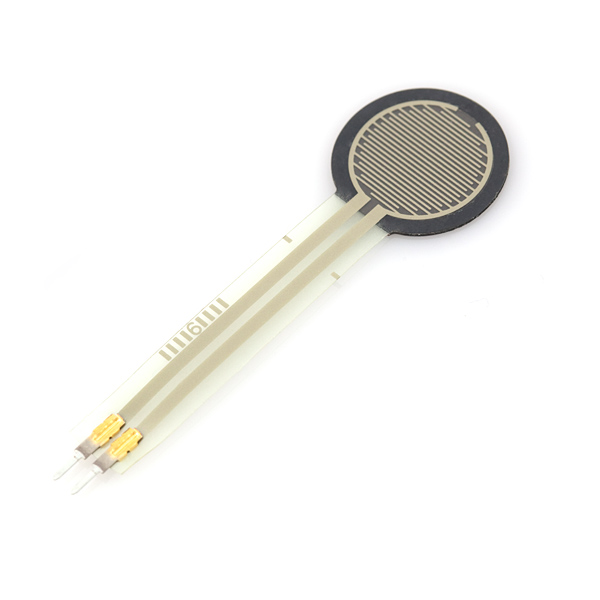
\includegraphics[width=0.25\textwidth]{chapter2/images/FSRx.jpg}
    \caption{ลักษณะโครงสร้างของตัวตรวจจับแรงกด FSR}
    \label{fig:fsr_sensor}
\end{figure}

\begin{figure}[H]
    \centering
    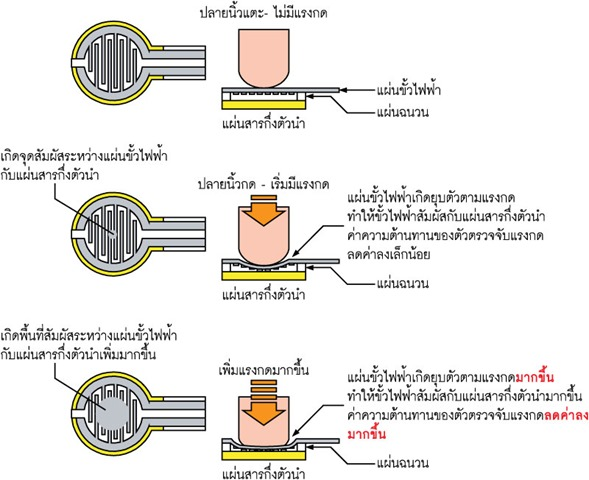
\includegraphics[width=0.65\textwidth]{chapter2/images/FSR.jpg}
    \caption{การทำงานของตัวตรวจจับแรงกด FSR}
    \label{fig:fsr_sensor_2}
\end{figure}

\subsubsection{เซนเซอร์วัดความเฉื่อย}

\begin{figure}[H]
    \centering
    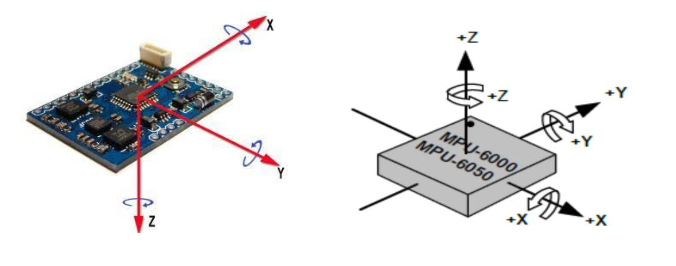
\includegraphics[width=0.65\textwidth]{chapter2/images/imu.png}
    \caption{เซนเซอร์วัดความเฉื่อย}
    \label{fig:imu_sensor}
\end{figure}

Inertial Measurement Unit (IMU) เป็นส่วนประกอบหลักที่ใช่ในการนำร่องเครื่องบิน ยาน-อวกาศ ดาวเทียม เรือ
ขีปนาวุธ ซึ่งในตัวของ IMU ประกอบไปด้วยสองส่วนหลักคือ Accelerometers 3 ทิศทาง ในการรับความเร่งเชิงเส้น
และ Gyroscopes 3 ทิศทาง ในการบอกความเร็วเชิงมุม เซนเซอร์ตัวนี้สามารถนำมาใช้ในการหาทิศทางการหมุนของตัวหุ่นยนต์ฮิวมานอยด์ได้

เซนเซอร์วัดความเร็ว (Gyroscope) เป็นอุปกรณ์สำหรับการวัดความเร็ว หรือการรักษาการปรับทิศทาง ขึ้นอยู่กับหลักการของการอนุรักษ์โมเมนตัมเชิงมุม
ถ้าไม่มีการเคลื่อนที่ อัตราการเปลี่ยนแปลงมุมจะมีค่าเท่ากับศูนย์

เซนเซอร์วัดความเร่ง (Accelerometer) เป็นอุปกรณ์ที่ใช้วัดความเร่งเชิงเส้น โดยอาศัยการวัดแรงที่กระทำต่อน้ำหนัก
อ้างอิงที่เกิดจากแรงโน้มถ่วงโลก ซึ่งแรงโน้มถ่วงของโลกจะเป็นเวกเตอร์ชี้ไปที่แกนกลางโลกเสมอ ตามกฎของนิวตัน

\subsection{แนวคิดการออกแบบกลไกการเดินของหุ่นยนต์ฮิวมานอยด์}
การออกแบบหุนยนตฮิวมานอยด์ใหสามารถเดินสองขาไดเสมือนมนุษยโดยใชจํานวนองศาอิสระใหเท่ากับมนุษยนั้นพบวา
มีขอจํากัดทางดานการออกแบบอยู่มาก เนื่องมาจากอุปกรณที่ใชในการขับเคลื่อนขอตอตางๆ มีอยูอยางจํากัด
รวมถึงขอจํากัดทางดานตัวรับรูตัวขับของหุนยนต ดังนั้นผูจัดทําจึงออกแบบหุนยนตใหมีองศาอิสระของขอตอ ในขาหนึ่งขาง
เทากับหกองศาอิสระ ทั้งนี้หุนยนตยังสามารถเคลื่อนที่ไดในปริภูมิ และองศาอิสระเพียงพอตอการใชงาน